\begin{appendices}
%Material that is complementary to the main body of the report can be included in an appendix. For externally sponsored students, if a report has been submitted to the sponsor during the year of the review, the report should be included in the appendix (a copy of the report can be supplied by the PGR coordinator). The appendix should include a list of training courses (including dates, duration, etc.) taken by the student during the year and other relevant research activities such as given seminars, attendance and presentations to conferences, etc. The appendix could also include material that is supplementary to the main body of the report such as: description of data sets, detailed experimental results, papers that have been submitted or published, etc.

\chapter{Gantt-Chart}
\label{app:gantt}

\chapter{Functional Reactive ABS (FrABS)}
\label{app:frABS}.
In this chapter we present our approach to implementing ABS in the pure functional language Haskell and discuss the issues encountered \footnote{This is not a real paper but only a basic introduction to our approach written for this 1st year report. Thus we assume knowledge of the concept of an agent and ABS already and won't explain these concepts again.}. As already described in our aims and objectives in Chapter \ref{chap:aimsObj}, we are using the functional reactive programming (FRP) paradigm as implemented by the library Yampa and implement an ABS library on top of it \footnote{We have implemented already a prototype together with the Sugarscape-, Agent\_Zero, SIRS- and Schelling-Segregation Model which can be accessed from \url{https://github.com/thalerjonathan/phd/tree/master/coding/libraries/frABS/examples}.}. When comparing our paradigms to the one of object-oriented Java we must solve fundamental problems in rather different ways.

\begin{enumerate}
	\item Representing an agent and environment - there are no classes and objects in Haskell.
	\item Interactions among agents and actions of agents on the environment - there are no method-calls and aliases in Haskell.
	\item Implement the necessary update-strategies as discussed in our paper \ref{app:updateStrategies}, where we only focus on sequential- and parallel-strategies - there is no mutable data which can be changed implicitly through side-effects (e.g. the agents, the list of all the agents, the environment).
\end{enumerate}

Before we can describe how we solved each of the problems, we first need to give an overview of the basic concepts of Yampa.

\section{Yampa}
The central concept of Yampa is the one of a signal-function which can be understood of a mapping from an input-signal to an output-signal. Whether the signal is discrete or continuous does not matter, Yampa is suited equally well to both kinds. Signal-functions are implemented in Yampa using continuations which allow to freeze program-state e.g. through closures and partial applications in functions which can be continued later:
\begin{lstlisting}[]
type DTime = Double

data SF a b = SF { sfTF :: DTime -> a -> (SF a b, b) }
\end{lstlisting}
Such a signal-function, which is called a \textit{transition function} in Yampa, takes the amount of time which has passed since the previous time step and the current input signal (a). It returns a \textit{continuation} of type SF a b determining the behaviour of the signal function on the next step and an output signal (b) of the current time-step. 

Yampa provides a top-level function, running in the IO-Monad, which drives a signal-function by providing both input-values and time-deltas from callbacks. It is important to note that when visualizing a simulation one has in fact two flows of time: the one of the user-interface which always follows real-time flow, and the one of the simulation which could be sped up or slowed down. Thus it is important to note that if I/O of the user-interface (rendering, user-input) occurs within the simulations time-frame then the user-interfaces real-time flow becomes the limiting factor. Yampa provides the function embedSync which allows to embed a signal function within another one which is then run at a given ratio of the outer SF. This allows to give the simulation its own time-flow which is independent of the user-interface. We utilized this in the implementation of Recursive ABS (see Chapter \ref{chap:work}).

Additional functionality which Yampa provides is the concept of Events which allow to implement changing behaviour of signal-functions at given points in time. An event can be understood to be similar to the Maybe-type of Haskell which either is an event with a given type or is simply NoEvent. Yampa provides facilities to detect if an event has fired and also provides functions to switch the signal-function into a new signal-function with changed behaviour. Another feature of Yampa is its EDSL for time-semantics: integration over time, delay, accumulation, holding, firing events after/now/repeatedly.

\section{Agent Representation}
An agent can be seen as a tuple $<id, s, m, ec, b>$.
\begin{itemize}
	\item \textbf{id} - the unique identifier of the agent
	\item \textbf{s} - the generic state of the agent
	\item \textbf{m} - the set of messages the agent understands
	\item \textbf{ec} - the \textit{type} of the environment-cells the agent may act upon
	\item \textbf{b} - the behaviour of the agent
\end{itemize}

\subsection{Id}
The id is simply represented as an Integer and must be unique for all currently existing agents in the system as it is used for message-delivery. A stronger requirement would be that the id of an agent is unique for the whole simulation-run and will never be reused - this would support replications and operations requiring unique agent-ids.

\subsection{State}
Each agent may have a generic state comprised of any data-type, most likely to be a structure.
\begin{lstlisting}[]
data SIRSState = Susceptible | Infected | Recovered
data SIRSAgentState = SIRSAgentState {
    sirsState :: SIRSState,
    sirsCoord :: SIRSCoord,
    sirsTime :: Double
} 
\end{lstlisting}

It is possible that the agent does not rely on any state s, then this will be represented by the unit type (). One wonders if this makes sense and asks how agents can then be distinguished between each other. In functional programming this is easily possible using currying and closures where one encapsulate initial state in the behaviour (see below), which allows to give each agent an individual initial state.

\subsection{Messages}
Agents communicate with each other through messages (see below) and thus need to have an agreed set of messages they understand. This is usually implemented as an ADT.
\begin{lstlisting}[]
data SIRSMsg = Contact SIRSState
\end{lstlisting}

\subsection{Environment-Cell}
The agent needs to know the generic type of the cells the environment is made of to be able to act upon the environment. Note that at the moment we only implemented a discrete 2d environment and provide only access and manipulation to the cells in a 2D discrete fashion. In the case of a continuous n-dimensional environment this approach needs to be thoroughly revised. It is important to understand that it is the \textit{type} of the cells and not the environment itself.

\subsection{Behaviour}
The behaviour of the agent is a signal-function which maps an AgentIn-Signal to an AgentOut-Signal. It has the following signature: 
\begin{lstlisting}[]
type AgentBehaviour s m e = SF (AgentIn s m e) (AgentOut s m e)
\end{lstlisting}

AgentIn provides the necessary data to the agent-behaviour: its id, incoming messages, the current state s, the environment (made out of the cells ec), its position in the environment and a random-number generator. 

AgentOut allows the agent to communicate changes out of the behaviour: kill itself, create new agents, sending messages, state s, environment (made out of the cells ec), environment-position and random-number generator. 

\section{Environment}
So far we only implemented a 2d-discrete environment. It can be understood to be a tuple of $<b, l, n, w, cs>$.
\begin{itemize}
	\item \textbf{b} - the optional behaviour of the environment
	\item \textbf{l} - the limit of the environment: its maximum boundary extending from (0,0)
	\item \textbf{n} - the neighbourhood of the environment (e.g. Neumann, Moore, Manhattan...)
	\item \textbf{w} - the wrapping-type of the environment (clipping, horizontal, vertical, both)
	\item \textbf{cs} - the cells of the environment of type c
\end{itemize}

We represent the environment-behaviour as a signal-function as well but one which maps an environment to itself. It has the following signature:
\begin{lstlisting}[]
type EnvironmentBehaviour c = SF (Environment c) (Environment c)
\end{lstlisting}
This is a regular SF thus having also the time of the simulation available and is called after all agents are updated. Note that the environment cannot send messages to agents because it is not an agent itself. An example of an environment behaviour would be to regrow some good on each cell according to some rate per time-unit (inspired by SugarScape regrowing of Sugar).

The cells are represented as a 2-dimensional array with indices from (0,0) to limit and a cell of type c at every position. Note that the cell-type c is the same environment-cell type ec of the agent.

Each agent has a copy of the environment passed in through the AgentIn and can change it by passing a changed version of the environment out through AgentOut.

\section{Messaging}
As discussed in the literature reflection in Chapter \ref{chap:refl}, inspired by the actor model we will resort to synchronized, reliable message passing with share nothing semantics to implement agent-agent interactions. Each Agent can send a message to an other agent through AgentOut-Signal where the messages are queued in the AgentIn-Signal and can be processed when the agent is updated the next time. The agent is free to ignore the messages and if it does not process them they will be simply lost.
Note that due to the fact we don't have method-calls in FP, messaging will always take some time, which depends on the sampling interval of the system. This was not obviously clear when implementing ABS in an object-oriented way because there we can communicate through method calls which are a way of interaction which takes no simulation-time.

%TODO: Push vs. Pull. we need push because we need to 'sample' the system at regular time-intervals because agent-behaviour can depend on time as well (pro-active) and not only on messaging. if we had only the latter, a pull approach would suffice.

% my wrongthinking: messaging ALWAYS takes time e.g. send/response roundtrip. conversations dont take time but are restricted for the receiver e.g. the receiver cannot send messages to others or change the environment in a conversation

% because an agent cannot reply within the same timestep sampling interval becomes an issue: if we need a reply within a given time then the sampling interval needs to be at least twice as much
% difference between discrete and continuous: the successor of discrete is defined whereas in the case of continuous it is not? how is the successor defined in the case of continuous time?

\section{Conversations}
The messaging as implemented above works well for one-directional, virtual asynchronous interaction where we don't need a reply at the same time. A perfect use-case for messaging is making contact with neighbours in the SIRS-model: the agent sends the contact message but does not need any response from the receiver, the receiver handles the message and may get infected but does not need to communicate this back to the sender. 
A different case is when agents need to transact in the time-step one or multiple times: agent A interacts with agent B where the semantics of the model (and thus messaging) need an immediate response from agent B - which can lead to further interactions initiated by agent A. The Sugarscape model has three use-cases for this: sex, warfare and trading amongst agents all need an immediate response (e.g. wanna mate with me?, I just killed you, wanna trade for this price?). The reason is that we need to transact now as all of the actions only work on a 1:1 relationship and could violate resource-constraints.
For this we introduce the concept of a conversation between agents. This allows an agent A to initiate a conversation with another agent B in which the simulation is virtually halted and both can exchange an arbitrary number of messages through calling and responding without time passing (something not possible without this concept because in each iteration the time advances). After either one agent has finished with the conversation it will terminate it and the simulation will continue with the updated agents (note the importance here: \textit{both} agents can change their state in a conversation). The conversation-concept is implemented at the moment in the way that the initiating agent A has all the freedom in sending messages, starting a new conversation,... but that the receiving agent B is only able to change its state but is not allowed to send messages or start conversations in this process. Technically speaking: agent A can manipulate an AgentOut whereas agent B can only manipulate its next AgentIn.
When looking at conversations they may look like an emulation of method-calls but they are more powerful: a receiver can be unavailable to conversations or simply refuse to handle this conversation. This follows the concept of an active actor which can decide what happens with the incoming interaction-request, instead of the passive object which cannot decide whether the method-call is really executed or not.

\section{Iteration-Strategies}
Building on the foundations laid out in my paper about iteration-strategies in Appendix \ref{app:updateStrategies}, we implement two of the four strategies: sequential- and parallel-strategy. We deliberately ignore the concurrent- and actor-strategy for now and leave this for further research \footnote{Also both strategies would require running in the STM-Monad, which is not possible with Yampa. The work of Ivan Perez in \cite{perez_functional_2016} implemented a library called Dunai, which is the same as Yampa but capable of running in an arbitrary Monad.}.
Implementing iteration-strategies using Haskell and FRP is not as straight-forward as in e.g. Java because one does not have mutable data which can be updated in-place. Although my work on programming paradigms in Appendix \ref{app:paradigms} did not take FRP into account, general concepts apply equally as well.

\subsection{Sequential}
In this strategy the agents are updated one after another where the changes (messages sent, environment changed,...) of one agent are visible to agents updated after. Basically this strategy is implemented as a variant of fold which allows to feed output of one agent (e.g. messages and the environment) forward to the other agents while iterating over the list of agents. For each agent the agent-behaviour signal-function is called with the current AgentIn as input to retrieve the according AgentOut. The messages of the AgentOut are then distributed to the receivers AgentIn.
The environment of the agent, which is passed in through AgentIn and returned through AgentOut will then be passed forward to all agents i + 1 AgentIn in the current iteration and override their old environment. Thus all steps of changes made to the environment are visible in the AgentOuts. The last environment is then the final environment in the current iteration and will be returned by the callback function together with the current AgentOuts.

\subsection{Parallel}
The parallel strategy is \textit{much} easier to implement than the sequential but is of course not applicable to all models because of it different semantics. Basically this strategy is implemented as a map over all agents which calls each agent-behaviour signal-function with the agents AgentIn to retrieve the new AgentOut. Then the messages are distributed amongst all agents.
A problem in this strategy is that the environment is duplicated to each agent and then each agent can work on it and return a changed environment. Thus after one iteration there are n versions of environments where n is equals to the number of agents. These environments must then be collapsed into a final one which is always domain-specific thus needs to be done through a function provided in the environment itself.

%TODO: functionsl approach to ABS: parallel application to previous states where only one agent is acting and the others are fixed. per step we have n results. for a full iteration we need $(n-1)^2$ applicatioms

\section{Further Research}
In his 1st year report about Functional Reactive GUI programming, Ivan Perez \footnote{main author of the paper \cite{perez_functional_2016}} writes: "FRP tries to shift the direction of data-flow, from message passing onto data dependency. This helps reason about what things are over time, as opposed to how changes propagate". This of course raises the question whether FRP is \textit{really} the right approach, because the way we implement ABS, message-passing is an essential concept. It is important to emphasis that agent-relations in interactions are never fixed in advance and are completely dynamic, forming a network. Maybe one has to look at message passing in a different way in FRP, and to view and model it as a data-dependency but it is not clear how this can be done. The question is whether there is a mechanism in which we have explicit data-dependency but which is dynamic like message-passing but does not try to fake method-calls? Maybe the concept of conversations (see above) are a way to go but we leave this for further research at the moment.

\chapter{Training Courses}
\label{app:courses}

\begin{itemize}
\item \textbf{Computer Science PGR Introductory Seminar} - 5 Dates
\item \textbf{Tradition of Critique Lecture series} - Monday 29th September 2016 to Monday 8th December 2016 (18:00 - 20:00)
\item \textbf{Graduate School}
	\begin{itemize}	
		\item Nature of the doctorate and the supervision process - 15th November 2016 (9:30 - 12:00)
		\item Presentation skills for researchers (all disciplines) - 27th Jan 2017 (9:30 - 15:30)
		\item Planning your research - 20th Feb 2017 (9:30 - 13:00)
		\item Getting into the habit of writing - 23rd Feb 2017 (9:30 - 12:30)
	\end{itemize}
\item \textbf{Midland Graduate School 2017} - 9th - 13th April 2017 in Leicester, courses in Denotational Semantics, Naïve Type Theory and Testing with Theorem Provers.
\end{itemize}

\chapter{Update-Strategies}
\label{app:updateStrategies}
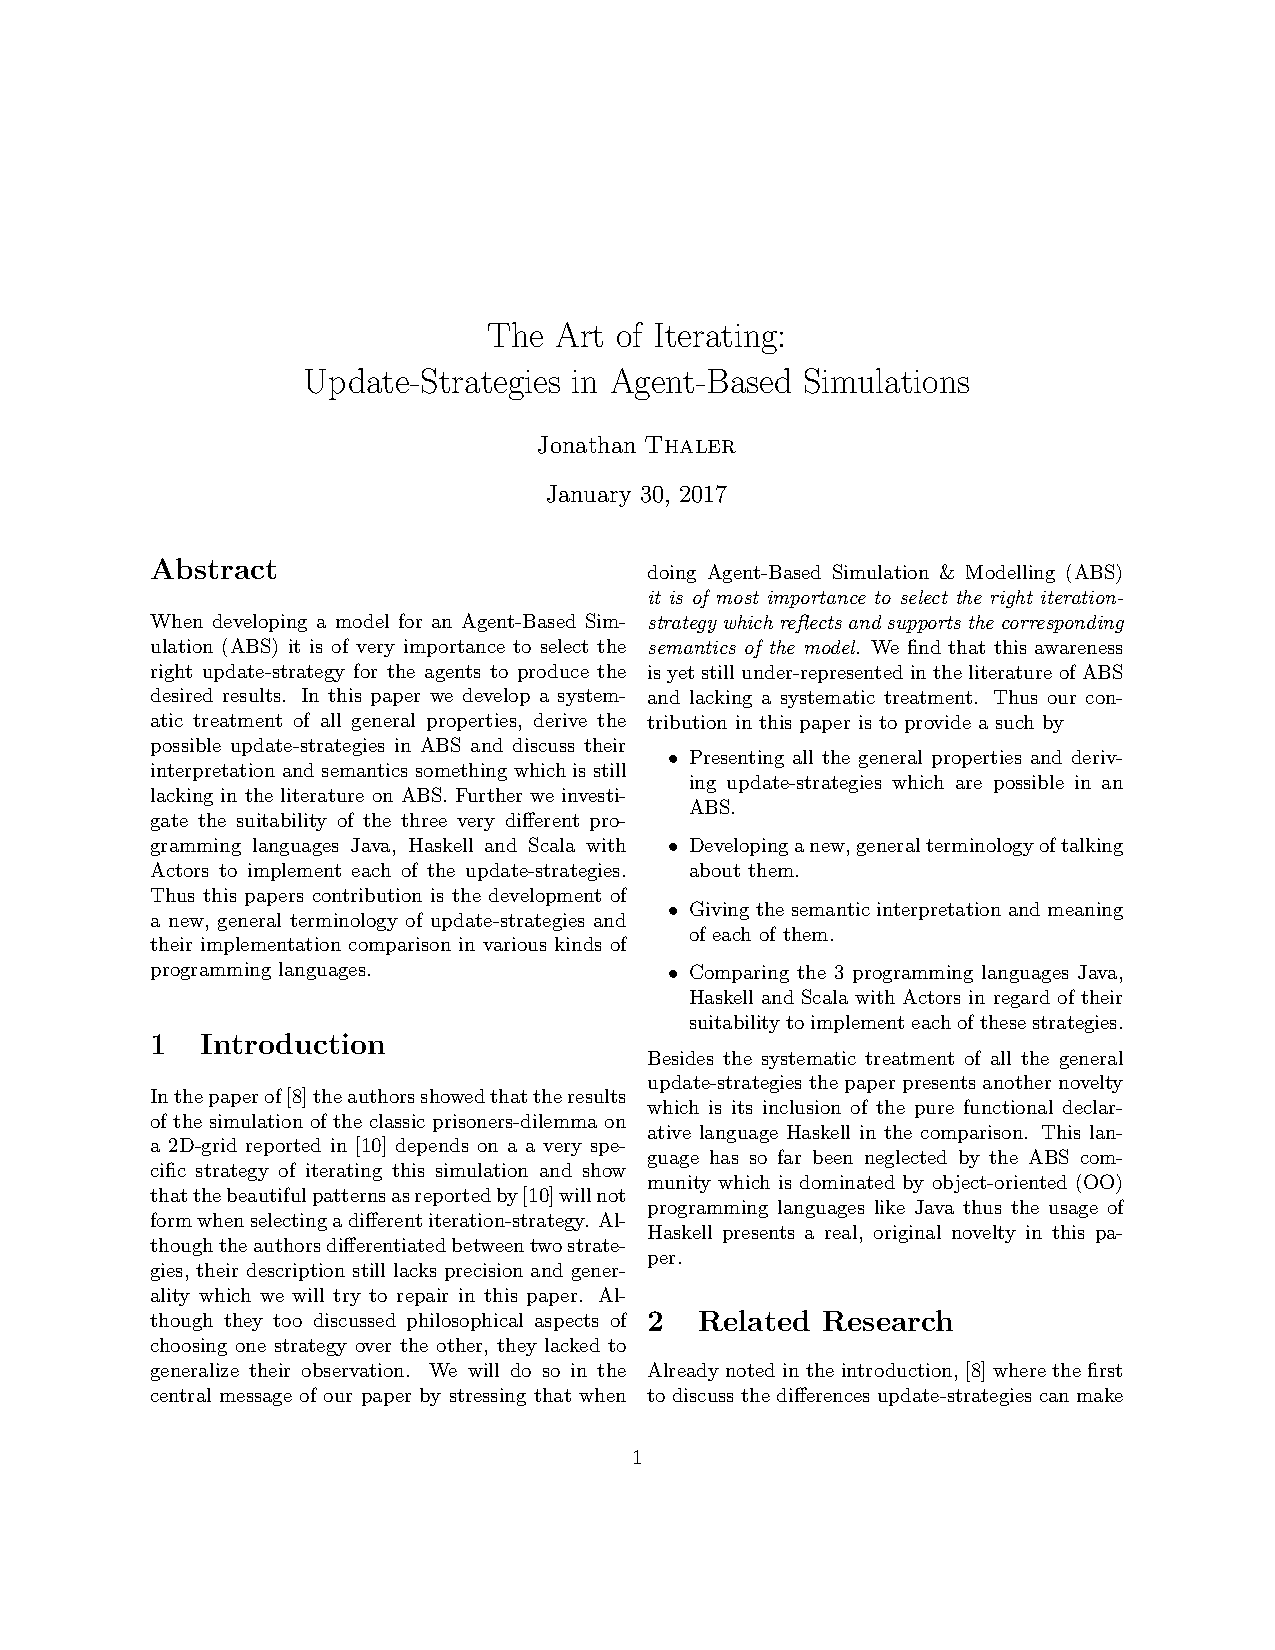
\includepdf[pages=-]{./pdf/iteratingABM.pdf}

\chapter{Programming-paradigms in ABS}
\label{app:paradigms}
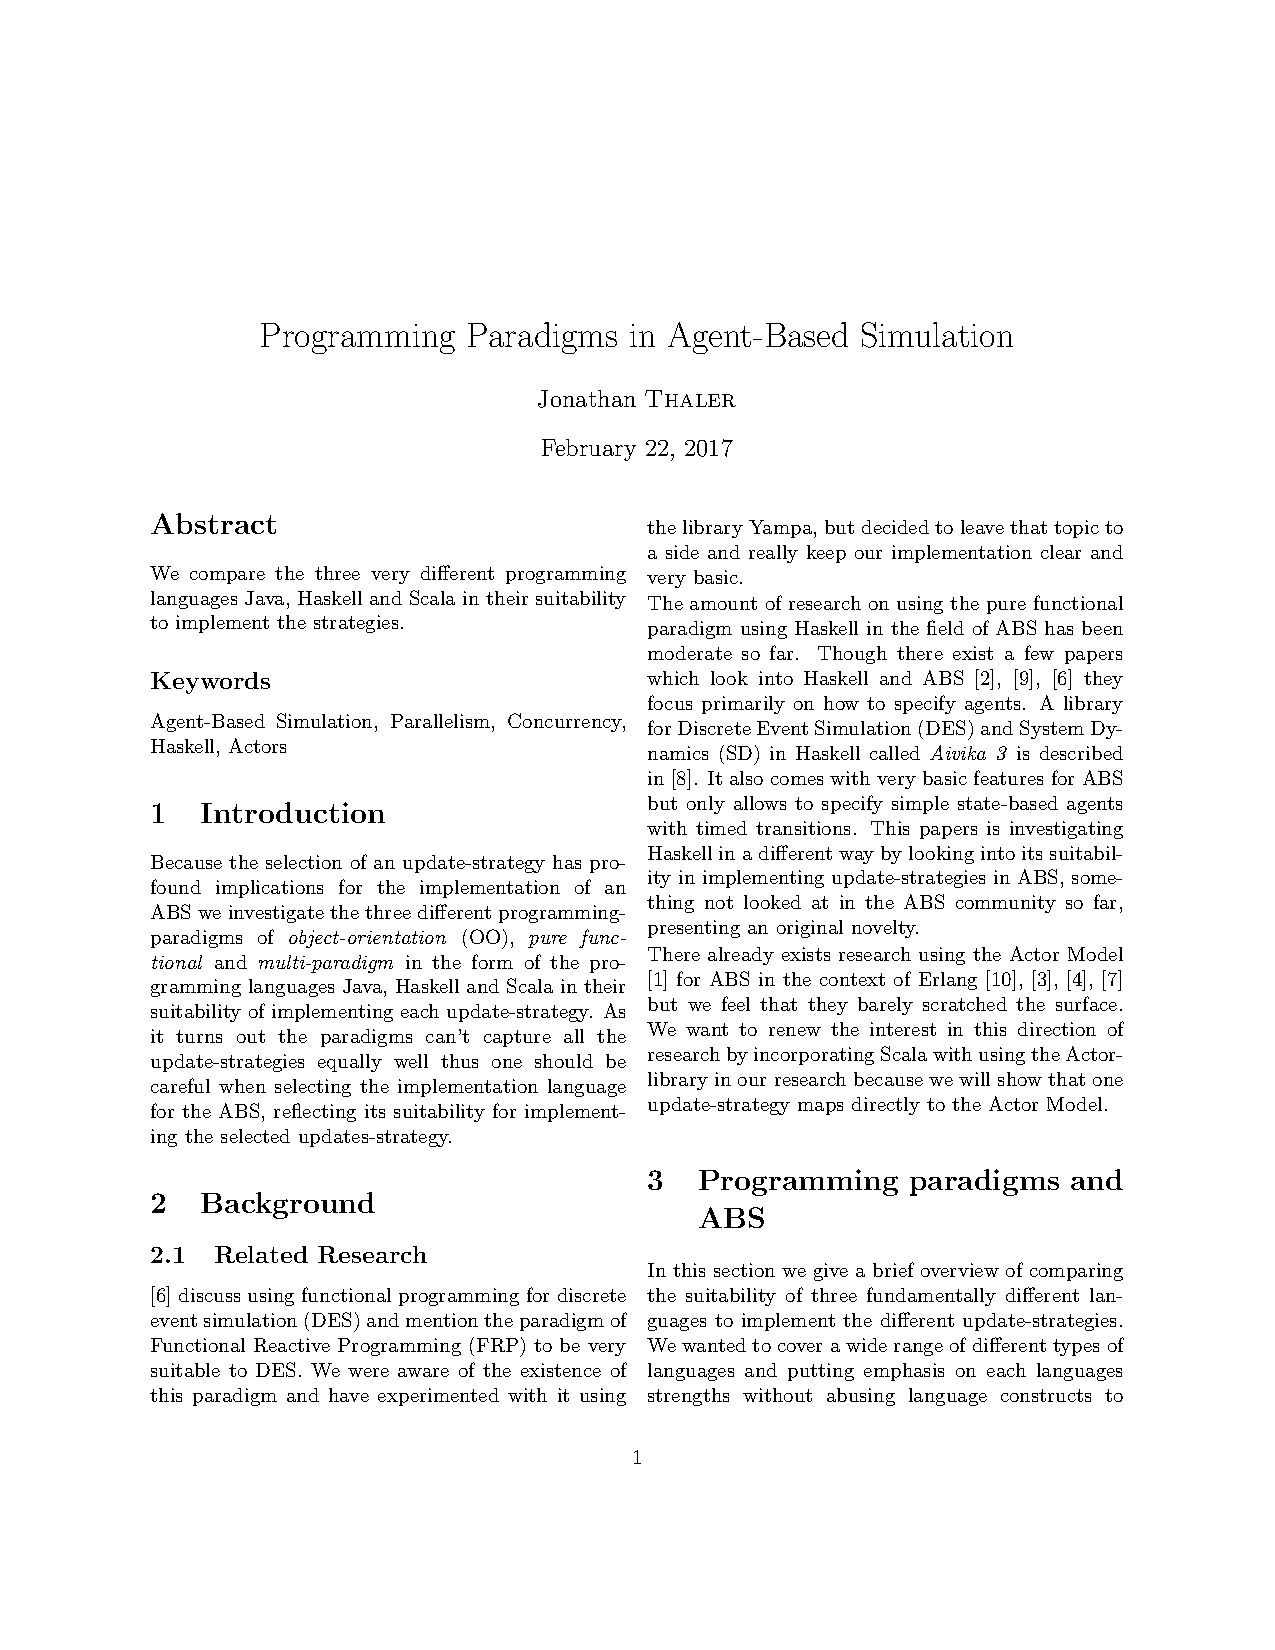
\includepdf[pages=-]{./pdf/programmingParadigmsABS.pdf}

\chapter{Questions \& Answers}
\label{chap:qa}

TODO: update and adopt to 2nd year

In this chapter I give answers to anticipated questions and objections about my research direction and vision of doing pure functional ABS \footnote{They are not always posed in a dead-serious way but as it is a quite controversial topic - ABS should be done object-orientated after all huh? - I think it is appropriate. Also some objections were raised in exactly this way.}.

\paragraph{So you had this hypothesis, that pure functional programming and dependent types lead to simulation software which is more likely correct and is easier to verify and validate, right from the beginning?}
Not at all. I even had no deep knowledge of functional programming at the start of my PhD, I've just worked through the 1st edition of Grahams book "Programming in Haskell" and that's it. I had no clear understanding of purity, side-effects and Monads and I didn't know a bit about functional reactive programming. I knew that something like Dependent Types exist because Thorsten (2nd Supervisor) has sent me an email before the start of my PhD in which he pointed at Agda, so I started reading a bit about intuitionistic / constructivistic math, tried out a little bit of Agda but quickly gave up because it was way too far away (without really having mastered pure functional programming in Haskell, I believe it is nearly impossible / too difficult / makes no sense going into dependent types).
So in the beginning there was pure \textit{curiosity} about functional programming in combination with ABS because I knew nothing of FP at all and wanted to understand it (after getting bored by OO) and applying FP to ABS seemed so crazy (because everyone claims OO to be 'natural' for it) that it must be an extremely interesting challenge. I guess this is very often the case with research: there is 'just' curiosity in the beginning and then during the research process a hypothesis falls into place.


\end{appendices}